\chapter{Cơ sở lý thuyết và các nghiên cứu liên quan}
\label{chap:background}

\section{Tổng quan các nghiên cứu liên quan}

Bài toán kiểm chứng trích dẫn tự động được xây dựng dựa trên ba lĩnh vực nền tảng của kỹ thuật phần mềm và xử lý ngôn ngữ tự nhiên (NLP): phân tích cú pháp tài liệu học thuật, liên kết bản ghi thư mục và phát hiện ảo giác trích dẫn. Mục này tổng hợp các hướng tiếp cận tiêu biểu trong từng lĩnh vực, đồng thời đặt các công cụ hiện có lên bàn cân so sánh trực tiếp với \textbf{CITRA}.

\subsection{Phân tích tài liệu và trích xuất tài liệu tham khảo}

Trích xuất thông tin trích dẫn có cấu trúc từ các tệp PDF chưa gán nhãn là chặng đầu tiên của mọi hệ thống kiểm tra danh mục tham khảo; bất kỳ sai sót nào phát sinh ở bước phân tích cú pháp đều sẽ lan truyền sang toàn bộ các mô-đun xử lý phía sau. Công cụ mã nguồn mở tiêu chuẩn hiện nay cho bài toán phân đoạn PDF khoa học là GROBID~\cite{Lopez2009}, sử dụng mô hình Trường ngẫu nhiên có điều kiện chuỗi tuyến tính (linear-chain CRF) để chuyển đổi các trang PDF thô sang tài liệu chuẩn Text Encoding Initiative XML (\texttt{TEI-XML}) bao gồm các đoạn văn thân bài, thẻ đánh dấu nội dòng \texttt{<ref type="bibr">} và các mục tham khảo có cấu trúc \texttt{<biblStruct>}. Mặc dù GROBID hoạt động rất hiệu quả trên các bài báo tạp chí được dàn trang chuẩn mực, các báo cáo đồ án tốt nghiệp của sinh viên xuất ra từ trình soạn thảo văn bản thường chứa mục lục trải dài nhiều dòng, thụt lề thiếu nhất quán hoặc các trích dẫn văn bản pháp luật Việt Nam khiến mô hình CRF thuần túy dễ phân loại nhầm hoặc cắt cụt nội dung.

Khi thiếu vắng các thẻ cấu trúc rõ ràng, nhóm bộ đọc PDF nhận biết bố cục trang đóng vai trò dự phòng thiết yếu. Thư viện PyMuPDF~\cite{PyMuPDF2024} trích xuất nhanh các khối văn bản nhờ tầng liên kết ngôn ngữ C biên dịch sẵn, trong khi \texttt{pdfplumber}~\cite{Pdfplumber2024} cung cấp tọa độ chi tiết đến từng ký tự để khôi phục bố cục trang hai cột và kiểu thụt đầu dòng treo (hanging indent). \textbf{CITRA} kết hợp GROBID \texttt{0.9.1-crf} với bộ lọc mục lục tất định, làm giàu trường thông tin bằng biểu thức chính quy, cơ chế dự phòng PyMuPDF/\texttt{pdfplumber} và bộ đọc \texttt{python-docx} nguyên bản nhằm đảm bảo các lỗi trình bày thường gặp ở báo cáo sinh viên không làm gián đoạn quá trình kiểm chứng.

\subsection{Liên kết bản ghi thư mục}

Bài toán liên kết bản ghi xác định liệu hai bản ghi siêu dữ liệu có nhiễu có cùng trỏ về một ấn phẩm thực tế duy nhất hay không. Fellegi và Sunter~\cite{Fellegi1969} đã đặt nền móng xác suất cho bài toán phân giải thực thể khi chứng minh rằng việc kết hợp đối chiếu độc lập trên nhiều trường thông tin (tiêu đề, họ tác giả, năm xuất bản và nơi công bố) mang lại tỷ lệ lỗi thấp hơn hẳn so với phép so khớp một chuỗi văn bản nối gộp duy nhất. Quan trọng không kém là tính bất đối xứng của bằng chứng phủ định: sự mâu thuẫn trực tiếp giữa hai trường đã có dữ liệu (chẳng hạn một mã DOI hợp lệ nhưng lại phân giải ra một tiêu đề hoàn toàn không liên quan) là bằng chứng mạnh mẽ khẳng định trích dẫn đã bị làm sai lệch, trong khi việc khuyết thiếu trường tên tạp chí hay hội nghị chỉ đơn thuần làm giảm độ tự tin của phép khớp. Sự phân biệt cốt lõi này chính là động lực để \textbf{CITRA} thiết kế hệ thống luật phân cấp theo thứ tự ưu tiên, trong đó kiểm tra các mâu thuẫn tường minh về định danh và trạng thái rút bài trước khi chấm điểm độ tương đồng siêu dữ liệu từng phần.

\subsection{Phát hiện trích dẫn ảo giác so với quy kết văn bản do AI sinh ra}

Các giải pháp ứng phó với tình trạng lạm dụng LLM trong giáo dục hiện nay đi theo hai hướng tiếp cận khác biệt về bản chất, được đối chiếu trực quan trong Hình~\ref{fig:verification-paradigm}. Hướng tiếp cận thứ nhất, \emph{quy kết theo phong cách hành văn}, huấn luyện các bộ phân loại thống kê hoặc bộ dò thủy vân số (watermark) nhằm ước lượng xác suất một đoạn văn bản được sinh ra bởi mô hình AI~\cite{Sculley2015}, \cite{Goodfellow2016}. Tuy nhiên, Sadasivan và cộng sự~\cite{Sadasivan2023} đã chứng minh cả về mặt lý thuyết lẫn thực nghiệm rằng các phép diễn đạt lại câu chữ dễ dàng đẩy độ chính xác của các bộ dò phong cách văn bản về mức đoán mò ngẫu nhiên. Krishna và cộng sự~\cite{krishna2023paraphrasing} tiếp tục khẳng định việc diễn đạt lại ở cấp độ diễn ngôn có thể qua mặt cả các công cụ phát hiện AI thương mại lẫn kỹ thuật đóng dấu thủy vân, đồng thời chỉ ra rằng phương pháp kiểm chứng dựa trên truy hồi nguồn đối chứng vẫn giữ được độ vững chắc cao. Hơn thế nữa, các công cụ đo lường phong cách chỉ khảo sát phân phối từ vựng trên bề mặt nên hoàn toàn không thể xác định liệu bài báo được trích dẫn có thực sự tồn tại hay không; mặt khác, sự mất cân bằng lớp trong các khóa sinh viên thực tế còn làm phình đại tỷ lệ báo động giả~\cite{Chawla2009}.

\begin{figure}[H]
    \centering
    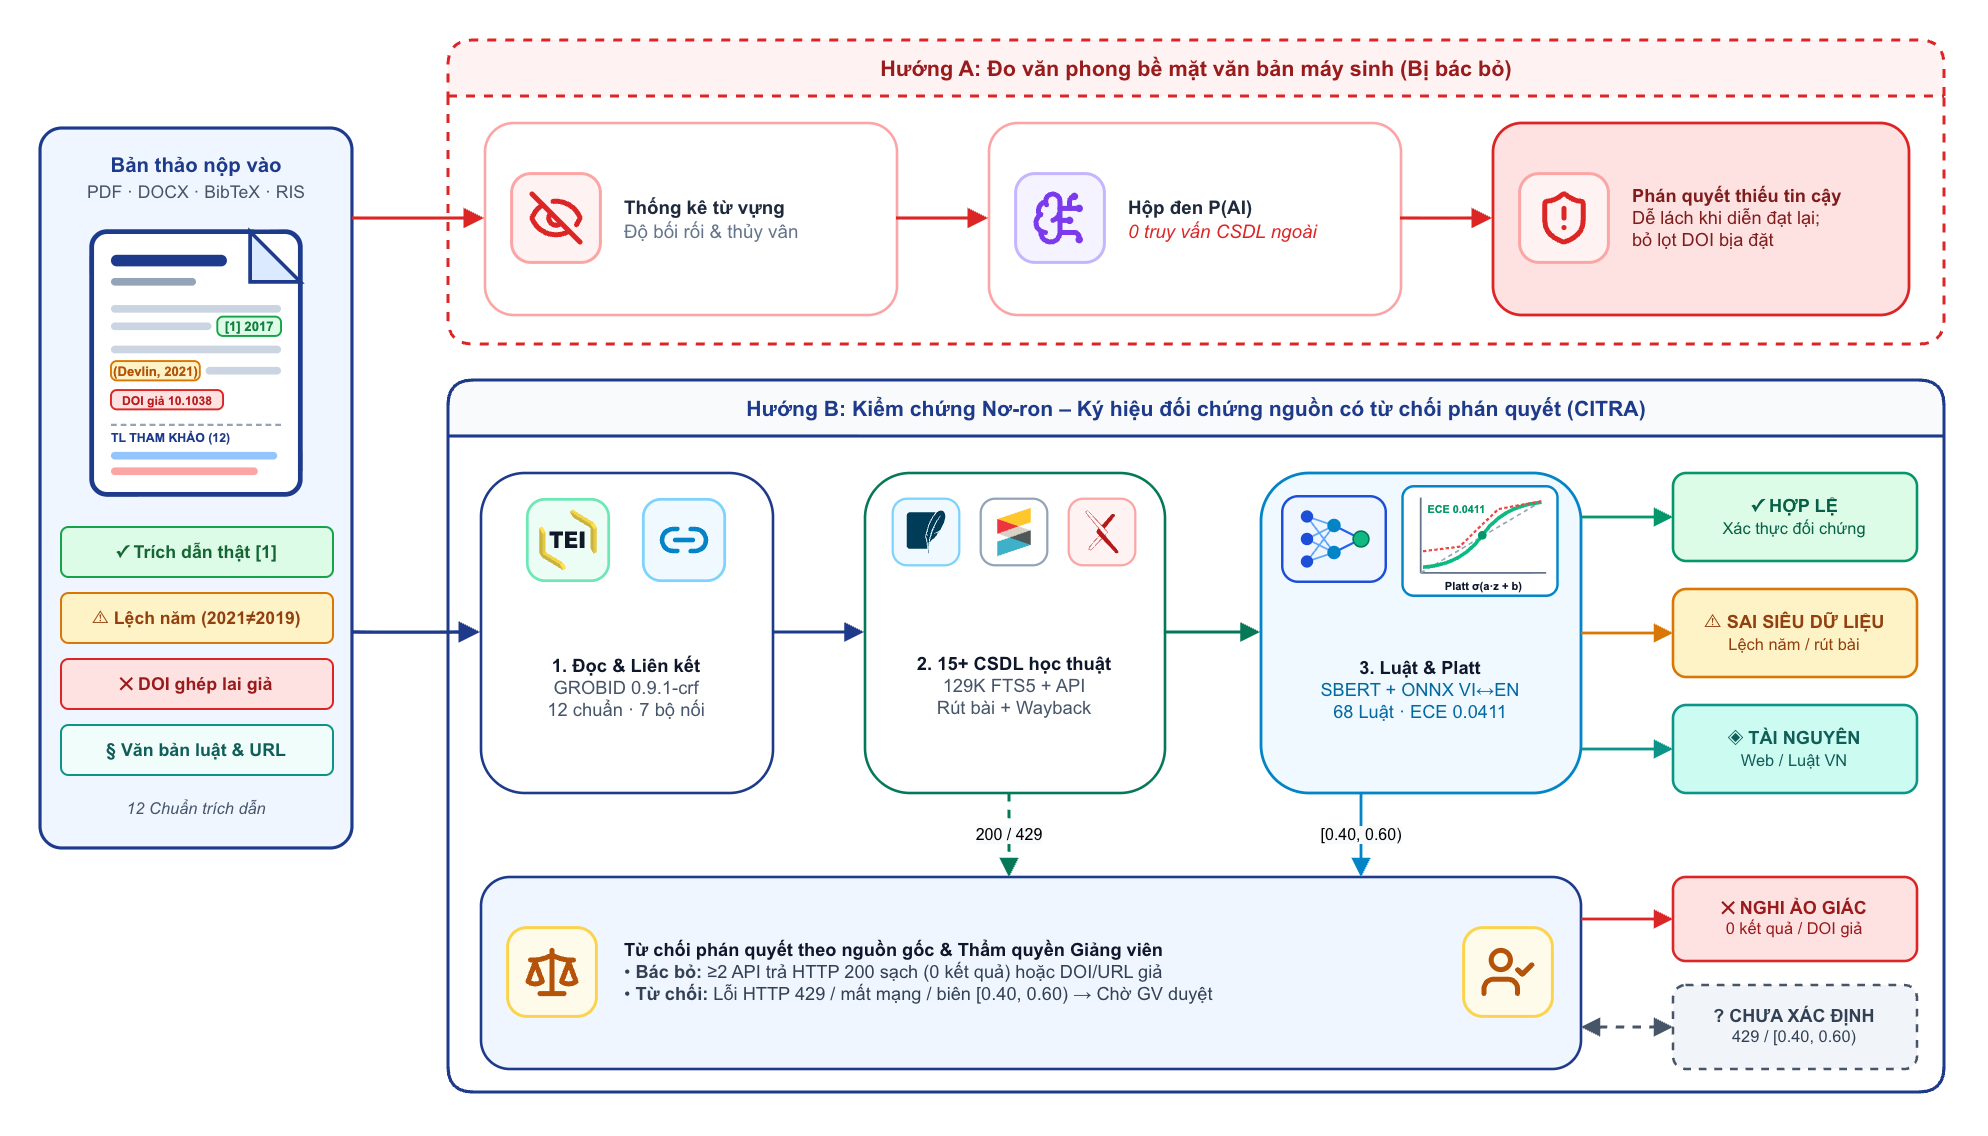
\includegraphics[width=\textwidth,keepaspectratio]{picture/figures/fig2_1_verification_paradigm.png}
    \caption[So sánh giữa quy kết theo phong cách hành văn và kiểm chứng thư mục đối chứng bên ngoài]{So sánh giữa phương pháp quy kết văn bản máy sinh theo phong cách hành văn và phương pháp kiểm chứng thư mục bên ngoài kết hợp từ chối phán quyết có chọn lọc dựa trên nguồn gốc.}
    \label{fig:verification-paradigm}
\end{figure}

Hướng tiếp cận thứ hai, \emph{kiểm chứng thư mục bên ngoài và đối sánh nhận định}, tra cứu từng trích dẫn trực tiếp trên các cơ sở dữ liệu có thẩm quyền và so sánh nội dung nhận định trong bài với bằng chứng truy hồi được, kế thừa tư tưởng của các khung kiểm chứng sự thật như FEVER~\cite{thorne2018fever}, SciFact~\cite{wadden2020scifact} và các bộ chuẩn tạo sinh gắn kết trích dẫn như ALCE~\cite{gao2023alce}. Mọi cảnh báo được đưa ra theo hướng tiếp cận này đều dựa trên bằng chứng đối chứng cụ thể từ bên ngoài: hoặc nhiều cơ sở dữ liệu trực tuyến cùng xác nhận không tồn tại bản ghi nào tương ứng, hoặc bản ghi chuẩn truy hồi được vạch rõ một sai lệch cụ thể về siêu dữ liệu hay nội dung nhận định.

\subsection{So sánh với các hệ thống hiện có}

Các nền tảng kiểm tra liêm chính học thuật, trình quản lý tài liệu tham khảo và bộ dữ liệu chuẩn nghiên cứu hiện nay đều chỉ giải quyết được một phần riêng lẻ trong quy trình kiểm chứng bản thảo của sinh viên. Những công cụ kiểm tra đạo văn như Turnitin đối sánh độ trùng lặp câu chữ với các kho lưu trữ đóng nhưng không thể phát hiện các tài liệu tham khảo bịa đặt vốn không hề trùng lặp văn bản với bất kỳ ấn phẩm nào đã công bố. Các trình quản lý tài liệu tham khảo như Zotero hỗ trợ tác giả nhập siêu dữ liệu sạch từ mã DOI nhưng không kiểm toán tính nhất quán của trích dẫn trong thân bài hay quản lý nộp bài theo lớp học. Trong khi đó, các bộ chuẩn NLP trên kho dữ liệu đóng như SciFact~\cite{wadden2020scifact} chỉ kiểm chứng nhận định khoa học trên tập cố định gồm 5,000 bản tóm tắt mà không phân tích tệp PDF đa chuẩn hay truy vấn trực tiếp các cơ sở dữ liệu trực tuyến. Bảng~\ref{tab:related-work} đối sánh \textbf{CITRA} với năm nhóm hệ thống tiêu biểu trên bảy năng lực kỹ thuật cốt lõi.

{\setlength{\tabcolsep}{3.5pt}
\begin{longtable}{|L{0.22}|C{0.11}|C{0.11}|C{0.11}|C{0.12}|C{0.11}|C{0.11}|C{0.11}|}
\caption{So sánh tính năng giữa các nhóm công cụ hiện có và CITRA (\texttt{v3.90.3}).}\label{tab:related-work}\\
\hline
\textbf{Nhóm hệ thống} & \textbf{PDF đa chuẩn} & \textbf{Liên kết 2 phía} & \textbf{15+ API trực tuyến} & \textbf{Đối sánh nhận định} & \textbf{Từ chối an toàn} & \textbf{Xác suất hiệu chỉnh} & \textbf{Pháp luật VN} \\
\hline
\endfirsthead
\multicolumn{8}{l}{\itshape Bảng \thetable\ (tiếp theo trang trước)}\\
\hline
\textbf{Nhóm hệ thống} & \textbf{PDF đa chuẩn} & \textbf{Liên kết 2 phía} & \textbf{15+ API trực tuyến} & \textbf{Đối sánh nhận định} & \textbf{Từ chối an toàn} & \textbf{Xác suất hiệu chỉnh} & \textbf{Pháp luật VN} \\
\hline
\endhead
\hline
\multicolumn{8}{r}{\itshape Xem tiếp trang sau}\\
\endfoot
\hline
\endlastfoot
Công cụ so trùng văn bản (Turnitin / iThen\-ticate) & Một phần & Không & Không & Không & Không & Không & Không \\
\hline
Công cụ dò văn phong AI (GPTZero / Thủy vân) & Không & Không & Không & Không & Không & Một phần & Không \\
\hline
Công cụ kiểm tra bằng LLM thuần câu lệnh & Một phần & Không & Một phần & Một phần & Không & Không & Không \\
\hline
Trình quản lý trích dẫn (Zotero / GROBID) & Có & Không & Một phần & Không & Không & Không & Không \\
\hline
Bộ chuẩn kiểm chứng nhận định (SciFact / ALCE) & Không & Không & Không & Có & Một phần & Không & Không \\
\hline
\textbf{CITRA (\texttt{v3.90.3})} & \textbf{Có (12)} & \textbf{Có (8)} & \textbf{Có (15+)} & \textbf{VI$\leftrightarrow$EN} & \textbf{Có} & \textbf{Platt} & \textbf{Có} \\
\hline
\end{longtable}
}

\section{Cơ sở dữ liệu học thuật và định danh bền vững}

\subsection{Hệ thống nguồn dữ liệu thư mục liên hợp}

Các nghiên cứu trắc lượng thư mục quy mô lớn cho thấy sự chênh lệch đáng kể về độ bao phủ giữa từng cơ sở dữ liệu học thuật riêng lẻ xét theo lĩnh vực chuyên môn cũng như loại hình ấn phẩm~\cite{visser2021bibliographic}. Việc phụ thuộc vào một API duy nhất còn gây ra tình trạng nghẽn cổ chai nghiêm trọng do giới hạn tần suất truy vấn vào những đợt cao điểm sinh viên nộp bài. Vì lý do đó, \textbf{CITRA} kết hợp một kho dữ liệu toàn văn ngoại tuyến với cơ chế định tuyến nhận biết miền chuyên ngành trên hơn mười lăm cơ sở dữ liệu học thuật, kỹ thuật và lưu trữ trực tuyến, được tổng hợp chi tiết trong Bảng~\ref{tab:sources}.

\begin{longtable}{|L{0.27}|L{0.36}|L{0.37}|}
\caption{Các cơ sở dữ liệu học thuật và bộ kiểm tra được tích hợp trong tầng truy hồi của CITRA.}\label{tab:sources}\\
\hline
\textbf{Nguồn dữ liệu / Bộ kiểm tra} & \textbf{Phạm vi bao phủ chính} & \textbf{Vai trò trong đường ống xử lý} \\
\hline
\endfirsthead
\multicolumn{3}{l}{\itshape Bảng \thetable\ (tiếp theo trang trước)}\\
\hline
\textbf{Nguồn dữ liệu / Bộ kiểm tra} & \textbf{Phạm vi bao phủ chính} & \textbf{Vai trò trong đường ống xử lý} \\
\hline
\endhead
\hline
\multicolumn{3}{r}{\itshape Xem tiếp trang sau}\\
\endfoot
\hline
\endlastfoot
Kho cục bộ (\texttt{local\_papers.db}) & 129,125 bản ghi (128,105 bài báo duy nhất; 82,877 bản tóm tắt) từ ACL Anthology~\cite{acl-anthology} và arXiv & Tra cứu ngoại tuyến Tầng 0 dưới 100\,ms bằng SQLite FTS5 BM25 \\
\hline
Danh sách kinh điển (\texttt{\_KNOWN\_PAPERS}) & 101 công trình nền tảng thuộc lĩnh vực KHMT, AI, NLP và học sâu & Tra cứu tức thời Tầng 0 cho các bài báo kinh điển có tần suất trích dẫn cao \\
\hline
Crossref~\cite{crossref-tdm} \& Retraction Watch & Tạp chí bình duyệt, kỷ yếu hội nghị, chương sách và thông báo rút bài & Phân giải DOI Tầng 1, phân tích tóm tắt chuẩn JATS (Journal Article Tag Suite) và sàng lọc cờ \texttt{is\_retracted} \\
\hline
OpenAlex~\cite{openalex} & Đồ thị học thuật mở toàn cầu bao phủ tạp chí, bản tiền ấn phẩm và kho lưu trữ & Tra cứu siêu dữ liệu diện rộng Tầng 1 và tái tạo tóm tắt từ chỉ mục ngược \\
\hline
DataCite~\cite{datacite} \& Global DOI RA~\cite{doi-handbook} & Tập dữ liệu Zenodo/\allowbreak Figshare/\allowbreak OSF và các cơ quan cấp phát DOI khu vực (JaLC, CNKI, KISTI, mEDRA) & Phân giải DOI ngoài Crossref ở Tầng 1 và kích hoạt cơ chế từ chối an toàn \texttt{R-DOI-\allowbreak RA-\allowbreak NO-\allowbreak CSL} \\
\hline
DOAJ~\cite{doaj} \& OpenAIRE / HAL & Tạp chí truy cập mở (bao gồm các tạp chí khu vực châu Á), kho lưu trữ trường viện và bản tiền ấn phẩm & Kiểm chứng tạp chí truy cập mở và kho lưu trữ học thuật cấp cơ sở ở Tầng 1 \\
\hline
DBLP~\cite{dblp} \& arXiv API~\cite{arxiv-api} & Hội nghị/hội thảo chuyên đề khoa học máy tính và bản tiền ấn phẩm khối STEM & Định tuyến thư mục chuyên ngành KHMT/AI và tra cứu chính xác mã \texttt{arXiv} ở Tầng 1 \\
\hline
Europe PMC~\cite{europepmc} \& NCBI / bioRxiv & Cơ sở dữ liệu PubMed/\allowbreak MEDLINE ngành y sinh, lâm sàng, tâm lý học và bản tiền ấn phẩm khoa học sự sống & Tra cứu chuyên ngành khoa học sự sống và làm giàu bản tóm tắt ở Tầng 1 \\
\hline
OpenLibrary~\cite{openlibrary} \& Google Books & Giáo trình, sách chuyên khảo, siêu dữ liệu ISBN và các lần tái bản đa ấn bản & Kiểm chứng sách ở Tầng 1 và dung sai năm xuất bản giữa các lần tái bản \\
\hline
Hugging Face, IETF RFC, PyPI \& Wikidata & Mô hình/tập dữ liệu học máy, chuẩn Internet RFC, gói thư viện Python và OpenCitations & Kiểm chứng phần mềm, tiêu chuẩn kỹ thuật và dữ liệu trích dẫn mở ở Tầng 1 \\
\hline
Bộ định tuyến Serper / SerpAPI & Chỉ mục tìm kiếm học thuật trên web dự phòng & Tầng 2 dự phòng tùy chọn khi cả Tầng 0 và Tầng 1 đều không trả về ứng viên nào \\
\hline
HTTP + Wayback \texttt{Link\allowbreak Validator}~\cite{openlibrary} & Đích truy cập HTTP/HTTPS trực tiếp và các bản chụp lưu trữ CDX của Internet Archive & Kiểm tra song song tính khả dụng của URL, phát hiện trang lỗi Soft-404 qua siêu dữ liệu HTML và tra cứu bản lưu trữ \\
\hline
\end{longtable}

\subsection{Phân giải định danh DOI và sàng lọc bài báo bị rút lại}

Định danh đối tượng số (DOI) cung cấp một mã tham chiếu bền vững cho các ấn phẩm học thuật~\cite{doi-handbook}, tuy nhiên việc đúng định dạng cú pháp (\texttt{10.xxxx/...}) hoàn toàn không bảo chứng cho tính xác thực của nguồn tài liệu. Các mô hình tạo sinh thường xuyên tự ghép các hậu tố chưa từng đăng ký vào sau những tiền tố có thật của nhà xuất bản uy tín (chẳng hạn \texttt{10.1109/}), hoặc sao chép mã DOI thật của một công trình nổi tiếng rồi gắn vào một mục trích dẫn bịa đặt. Ở chiều ngược lại, nhiều tạp chí hợp pháp tại châu Á hoặc châu Âu đăng ký qua các cơ quan cấp phát khu vực như JaLC, CNKI, KISTI hay mEDRA vẫn phân giải hợp lệ tại \texttt{doi.org/ra/} dù không công bố siêu dữ liệu trên Crossref. Việc truy vấn trực tiếp API của Cơ quan đăng ký DOI toàn cầu (Global DOI RA) giúp \textbf{CITRA} từ chối phán quyết một cách an toàn đối với các mã DOI khu vực hợp lệ, đồng thời vạch trần chính xác các mã DOI chưa đăng ký hoặc bị gắn ghép chắp vá. Song song đó, bước đối chiếu trường cập nhật siêu dữ liệu (\texttt{update-to}) trên Crossref kết hợp cùng danh sách cảnh báo từ Retraction Watch ngăn chặn triệt để việc các bài báo đã bị rút lại lọt qua hệ thống như những nguồn tài liệu hợp lệ.

\section{Cơ sở lý thuyết và mô hình toán học}

\subsection{Độ tương đồng tiêu đề theo từ vựng và ngữ nghĩa}

Chuỗi thông tin thư mục của cùng một công trình thường biến thiên đáng kể giữa các chuẩn trích dẫn do việc lược bỏ tiêu đề phụ, khác biệt dấu câu, dấu gạch nối hoặc ký hiệu lần xuất bản. Do đó, \textbf{CITRA} kết hợp phép đo độ tương đồng chuỗi ở mức từ vựng với biểu diễn nhúng nơ-ron dày đặc. Ở tầng từ vựng, thư viện RapidFuzz tính toán tỷ lệ tập từ khóa (token-set ratio, bất biến với sự thay đổi trật tự từ), tỷ lệ khoảng cách Levenshtein chuẩn hóa (nhạy với lỗi chính tả ký tự) và tỷ lệ tiền tố có kiểm soát (xử lý trường hợp lược bỏ tiêu đề phụ sau dấu hai chấm). Ở tầng ngữ nghĩa, các tiêu đề được mã hóa thành những véc-tơ 384 chiều dựa trên kiến trúc Transformer~\cite{vaswani2017} đã chưng cất tri thức qua BERT~\cite{bert} và MiniLM~\cite{wang2020minilm} thành mô hình Sentence-BERT \texttt{all-MiniLM-L6-v2}~\cite{reimers2019sbert}. Khi văn bản thân bài tiếng Việt trích dẫn một tài liệu nguồn tiếng Anh, \textbf{CITRA} tự động kích hoạt bộ mã hóa đa ngữ lượng tử hóa ONNX INT8 (\texttt{paraphrase-multilingual-MiniLM-L12-v2}) được huấn luyện bằng kỹ thuật chưng cất tri thức đa ngôn ngữ~\cite{reimers2020multilingual}.

\subsection{Đối sánh ngữ cảnh đa câu}

Việc chỉ kiểm tra siêu dữ liệu ở danh mục tham khảo không thể phát hiện lỗi \emph{gán ghép sai ngữ cảnh}, tức trường hợp sinh viên trích dẫn một bài báo có thật để củng cố cho một nhận định không liên quan hoặc thậm chí trái ngược với nội dung bài báo gốc. Tuy nhiên, nếu đem một câu trích dẫn đơn lẻ trong thân bài so sánh trực tiếp với toàn bộ phần tóm tắt dài khoảng mười câu, điểm tương đồng sẽ bị pha loãng do các câu giới thiệu bối cảnh và kết luận chung làm mờ đi câu phát hiện cụ thể đang được viện dẫn. Với ngữ cảnh trích dẫn trong bài $c$ và bản tóm tắt ứng viên $A$ được tách thành tập các câu $\{s_1, \dots, s_m\}$, \textbf{CITRA} tính điểm đối sánh tóm tắt gộp $s_{\text{abs}}(c, A)$ theo Phương trình~\eqref{eq:abs-pooling}:
\begin{equation}\label{eq:abs-pooling}
s_{\text{abs}}(c, A) = \max\Bigl(\cos\bigl(\mathbf{e}(c), \mathbf{e}(A)\bigr),\; 0.65 \max_{1 \le i \le m} \cos\bigl(\mathbf{e}(c), \mathbf{e}(s_i)\bigr) + 0.35 \cos\bigl(\mathbf{e}(c), \mathbf{e}(A)\bigr)\Bigr),
\end{equation}
trong đó $\mathbf{e}(\cdot)$ biểu thị véc-tơ nhúng câu đã chuẩn hóa L2. Phương trình~\eqref{eq:abs-pooling} vừa giữ được điểm tương đồng cao khi câu trích dẫn nhắm tới một kết quả cụ thể duy nhất trong bài báo, vừa bảo toàn ngữ cảnh tổng thể của toàn bộ bản tóm tắt khi sinh viên trích dẫn nhằm khái quát nội dung chung của công trình. Điểm đối sánh nội dung cuối cùng là tổ hợp có trọng số giữa độ tương đồng tiêu đề ($0.30$), độ tương đồng tóm tắt gộp ($0.50$) và độ tương đồng đoạn trích toàn văn ($0.20$, được chuẩn hóa lại trọng số khi không có toàn văn).

\subsection{Phân loại có chọn lọc và hiệu chỉnh xác suất Platt trên không gian logit}

Trong các hệ thống hỗ trợ ra quyết định có mức độ ảnh hưởng cao, một bộ phân loại phải biết thời điểm cần từ chối đưa ra phán quyết~\cite{chow1970optimum}, \cite{Geifman2017}, đồng thời độ tin cậy $p$ mà hệ thống công bố phải phản ánh sát xác suất đúng thực nghiệm~\cite{hand2009}, \cite{guo2017}. Độ tin cậy gán tĩnh theo luật thường co cụm tại một vài hằng số rời rạc và đánh giá quá cao mức độ chắc chắn ở vùng lân cận biên quyết định. Với nhãn kết luận ký hiệu $y_{\text{sym}}$ và véc-tơ đặc trưng 16 chiều $\mathbf{x} \in \mathbb{R}^{16}$, \textbf{CITRA} pha trộn độ tin cậy của luật ký hiệu $C_{\text{sym}}$ với xác suất dự đoán theo lớp $P_{\text{ML}}(y_{\text{sym}} \mid \mathbf{x})$ từ mô hình hồi quy logistic đa lớp thông qua trọng số $\alpha \in [0, 1]$, như định nghĩa tại Phương trình~\eqref{eq:platt-calib}:
\begin{equation}\label{eq:platt-calib}
p_{\text{blend}} = \alpha C_{\text{sym}} + (1 - \alpha) P_{\text{ML}}(y_{\text{sym}} \mid \mathbf{x}), \;\;
P_{\text{cal}} = \operatorname{clip}\!\left(\sigma\Bigl(a \cdot \ln\frac{\tilde{p}}{1 - \tilde{p}} + b\Bigr),\, 0.01,\, 0.99\right),
\end{equation}
trong đó $\tilde{p} = \min(\max(p_{\text{blend}}, 10^{-4}), 1 - 10^{-4})$ giúp ngăn hiện tượng tràn số học tại hai biên $0$ và $1$, $\sigma(z) = (1 + e^{-z})^{-1}$ là hàm sigmoid logistic, còn $(a, b)$ là cặp tham số vô hướng của phép hiệu chỉnh xác suất Platt~\cite{platt1999} được ước lượng trên tập kiểm định tách rời thông qua việc cực tiểu hóa hàm mục tiêu kết hợp giữa đối log hợp lý âm và điểm Brier~\cite{brier1950}.

\subsection{Thiết kế thực nghiệm phân tách độc lập theo bài báo gốc}

Tuân thủ các nguyên tắc thực nghiệm trong Kỹ thuật phần mềm thực nghiệm~\cite{wohlin2012experimentation} cũng như các bộ chuẩn kiểm chứng nhận định khoa học~\cite{thorne2018fever}, \cite{wadden2020scifact}, quá trình huấn luyện và đánh giá một bộ kiểm chứng lai đòi hỏi cơ chế bảo vệ nghiêm ngặt trước hiện tượng rò rỉ dữ liệu và nhiễu tạo tác trong tập dữ liệu~\cite{gururangan2018annotation}, \cite{poliak2018hypothesis}. Nếu các biến thể gây nhiễu sinh ra từ cùng một bài báo gốc đồng thời xuất hiện ở cả tập huấn luyện lẫn tập kiểm thử, bộ phân loại có thể học vẹt phân phối đặc trưng riêng của bài báo đó. Tương tự, nếu điểm ngữ cảnh ngữ nghĩa khác không chỉ xuất hiện ở các mẫu hợp lệ, mô hình sẽ dễ dàng học theo một đường tắt tầm thường thay vì hiểu bản chất bài toán. Vì vậy, toàn bộ thực nghiệm định lượng tại Chương~\ref{chap:results} đều phân hoạch nghiêm ngặt tập bài báo gốc trước khi sinh biến thể nhiễu, giữ nguyên biểu diễn mã hóa thực tế từ Sentence-BERT trên tất cả các lớp mà không gán ép nhân tạo, đồng thời kiểm định giả thuyết bằng phép kiểm McNemar có hiệu chỉnh liên tục~\cite{dietterich1998approximate}, phép điều chỉnh đa so sánh Holm--Bonferroni~\cite{holm1979simple} và kỹ thuật lấy mẫu lại bootstrap bắt cặp~\cite{bergkirkpatrick2012empirical}, \cite{dror2018hitchhiker}.

\section{Tóm tắt chương}

Chương này đã tổng quan các công trình nghiên cứu về phân tích trích dẫn trên tệp PDF, liên kết bản ghi thư mục theo xác suất và phát hiện tài liệu tham khảo ảo giác, đồng thời đối sánh \textbf{CITRA} với năm nhóm công cụ hiện có. Chương cũng đã làm rõ cơ sở của kiến trúc truy hồi liên hợp đa nguồn cũng như xây dựng mô hình toán học cho phép đối sánh ngữ nghĩa gộp theo câu và hiệu chỉnh xác suất Platt trên không gian logit. Chương~\ref{chap:overview} tiếp theo sẽ cụ thể hóa các nền tảng lý thuyết này thành đặc tả yêu cầu phần mềm hình thức, mô hình ca sử dụng, lược đồ cơ sở dữ liệu và kiến trúc triển khai hệ thống.
